\documentclass[tikz,border=8pt]{standalone}

\usepackage[T1]{fontenc}
\usepackage{lmodern}
\usepackage{tikz}
\usetikzlibrary{arrows.meta,calc,positioning}

% Ikran technical architecture — editable master figure.
% The diagram is intentionally implementation-agnostic: it explains the
% division of responsibilities and the three bidirectional relationships.

\definecolor{ink}{HTML}{1F2933}
\definecolor{muted}{HTML}{5E6B75}
\definecolor{line}{HTML}{697780}
\definecolor{nodefill}{HTML}{F7F8F9}
\definecolor{ikranfill}{HTML}{EDF4F7}
\definecolor{ikranline}{HTML}{3F6575}

\begin{document}
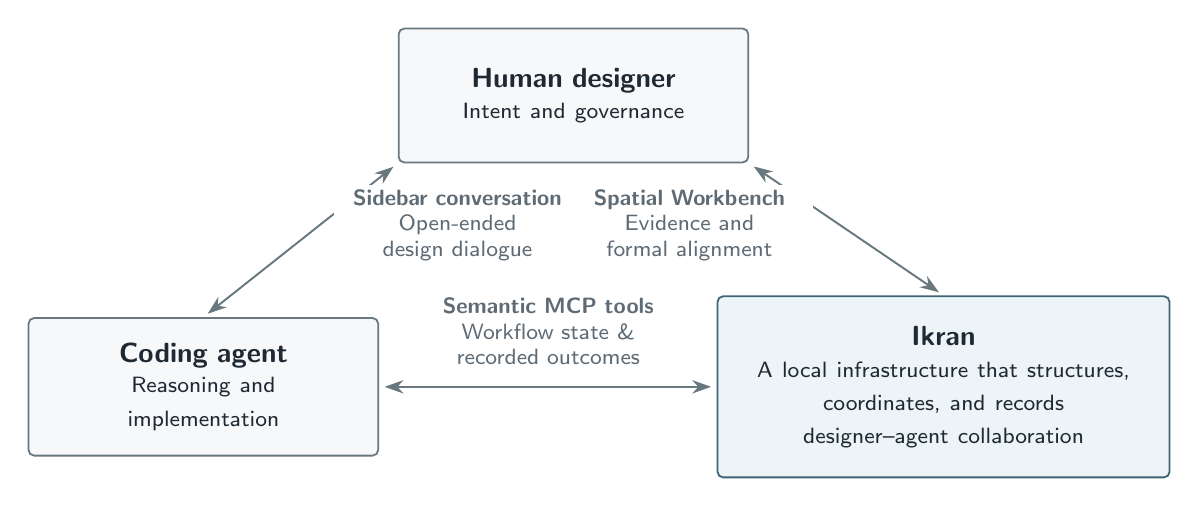
\begin{tikzpicture}[
  font=\sffamily,
  text=ink,
  >={Stealth[length=2.4mm,width=1.7mm]},
  actor/.style={
    draw=line,
    fill=nodefill,
    line width=0.65pt,
    rounded corners=2pt,
    align=center,
    text width=38mm,
    minimum height=17mm,
    inner sep=3.2mm
  },
  ikran/.style={
    actor,
    draw=ikranline,
    fill=ikranfill,
    text width=51mm,
    minimum height=23mm
  },
  relation/.style={
    <->,
    draw=line,
    line width=0.7pt,
    shorten <=2pt,
    shorten >=2pt
  },
  edge label/.style={
    align=center,
    fill=white,
    inner sep=2pt,
    text width=30mm,
    text=muted,
    font=\sffamily\fontsize{7.6}{9.2}\selectfont
  }
]

% Triangle vertices
\node[actor] (designer) at (0,3.7) {%
  {\fontsize{10}{12}\selectfont\bfseries Human designer}\\[-1pt]
  {\fontsize{8}{10}\selectfont Intent and governance}%
};

\node[actor] (agent) at (-4.7,0) {%
  {\fontsize{10}{12}\selectfont\bfseries Coding agent}\\[-1pt]
  {\fontsize{8}{10}\selectfont Reasoning and implementation}%
};

\node[ikran] (ikran) at (4.7,0) {%
  {\fontsize{10}{12}\selectfont\bfseries Ikran}\\[1.5pt]
  {\fontsize{8}{10}\selectfont A local infrastructure that structures,\\
  coordinates, and records designer--agent collaboration}%
};

% The three bidirectional relationships form the structural triangle.
\draw[relation] (designer.south west) -- (agent.north);
\draw[relation] (designer.south east) -- (ikran.north);
\draw[relation] (agent.east) -- (ikran.west);

% Horizontal labels remain legible at typical two-column publication size.
\node[edge label,anchor=west] at (-3.05,2.05) {\bfseries Sidebar conversation\\\mdseries Open-ended\\design dialogue};
\node[edge label,anchor=east] at (3.05,2.05) {\bfseries Spatial Workbench\\\mdseries Evidence and\\formal alignment};
\node[edge label,text width=36mm] at (-0.32,0.70) {\bfseries Semantic MCP tools\\\mdseries Workflow state \& recorded outcomes};


\end{tikzpicture}
\end{document}
